\documentclass[times, utf8, diplomski]{fer}
\usepackage{booktabs}
\usepackage{pdfpages}
\usepackage{listings}

\renewcommand{\lstlistingname}{Isječak}

\lstset{
	basicstyle=\linespread{1.2}\ttfamily\footnotesize,
	keepspaces=true,
	numbers=left,
	frame=single,
	captionpos=b,
	showspaces=false,
	numberstyle=\ttfamily,
	columns=flexible,
	extendedchars=true,
	inputencoding=utf8,
	xleftmargin=5mm,
	xrightmargin=5mm
}

\begin{document}

\thesisnumber{2565}

\title{Analiza performansi sustava za udaljeno izvršavanje programskog kôda}

\author{Herman Zvonimir Došilović}

\maketitle

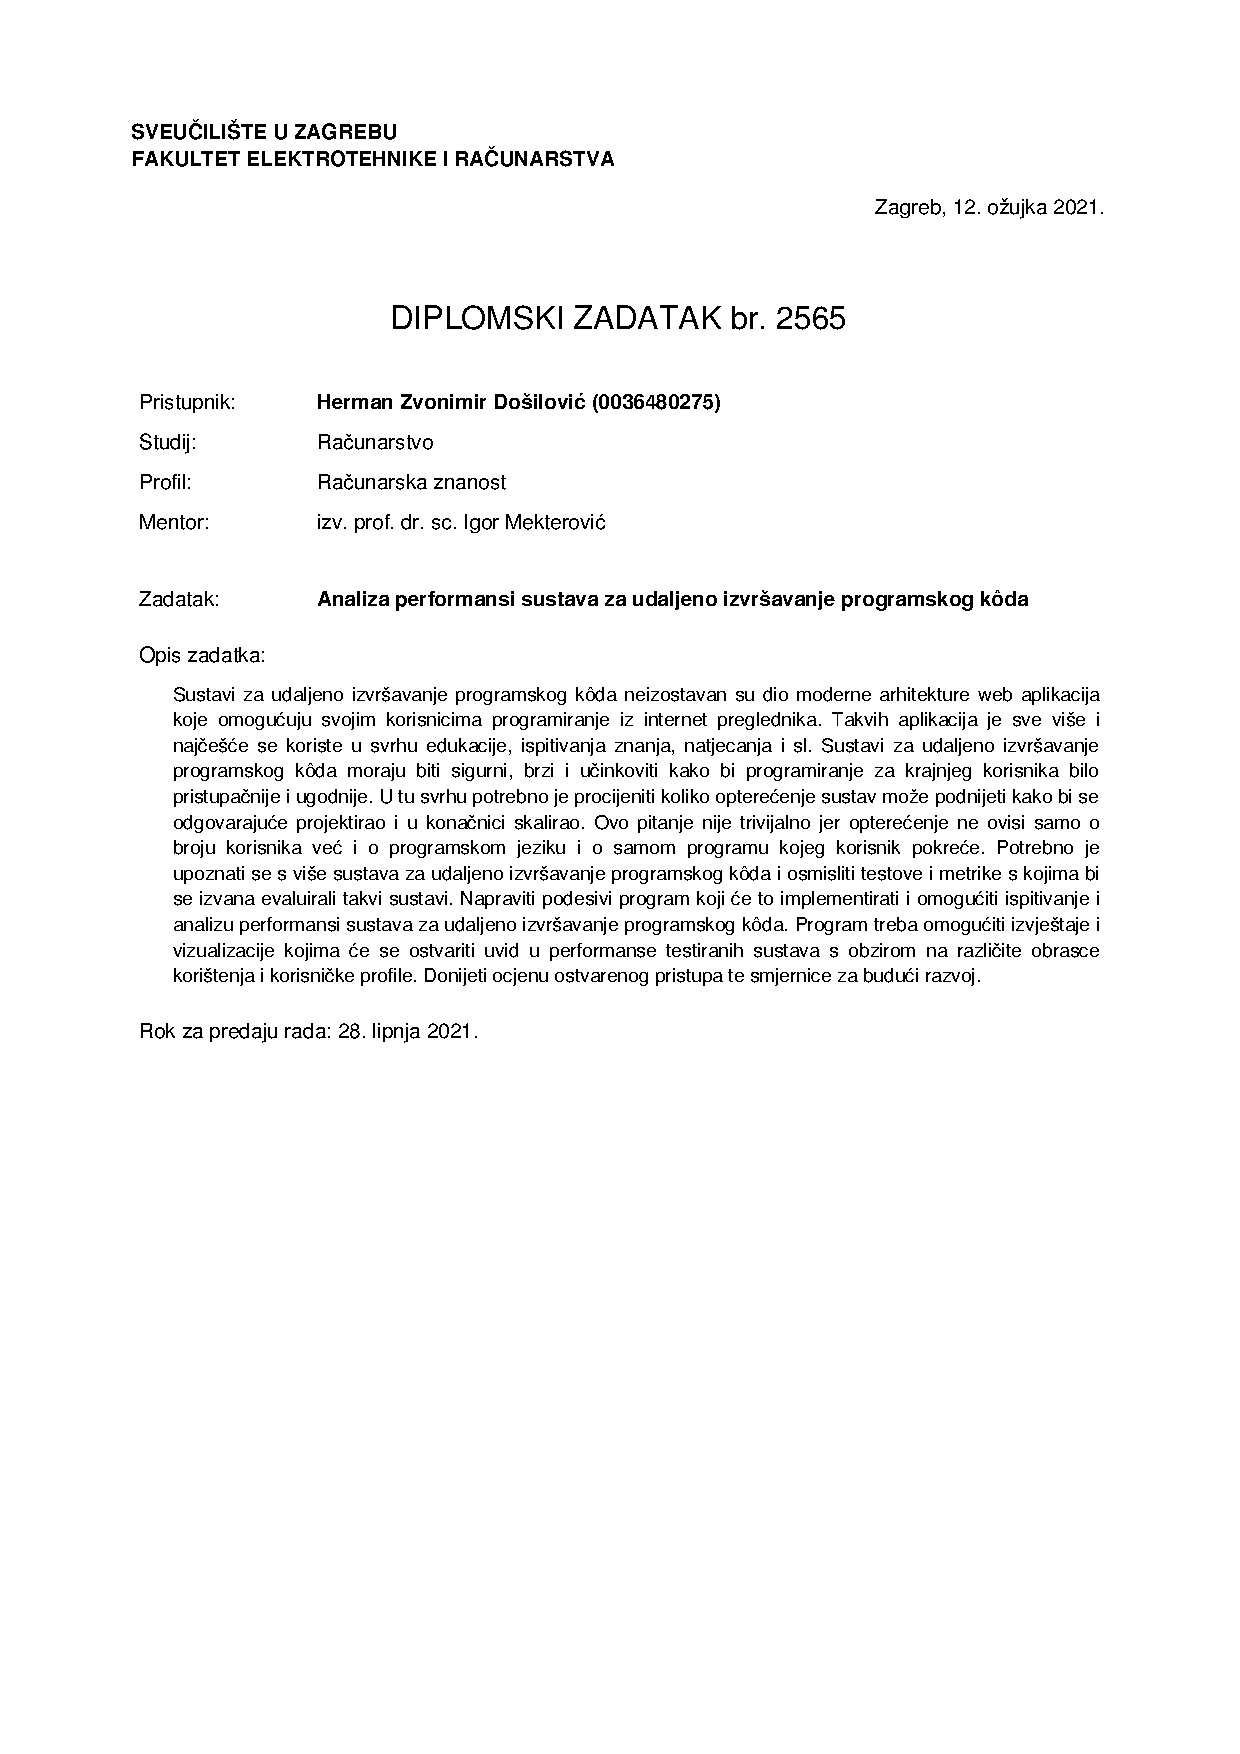
\includepdf[pages=-]{hr_0036480275_56.pdf}

\zahvala{}

\tableofcontents

\chapter{Uvod}

\chapter{Sustavi za udaljeno ocjenjivanje}
Sustav za udaljeno ocjenjivanje (engl.\ \textit{online judge}, krat.\ \textit{OJ}) je sustav za evaluaciju korisničkog programskog kôda na unaprijed zadanom skupu primjera za ispitivanje. Sustav za udaljeno ocjenjivanje koristi se u različitim slučajevima uporabe \engl{use-cases} kao što su npr.: natjecateljsko programiranje \engl{competitive programming}, e-učenje \engl{e-learning}, i u regrutiranju i procesu zapošljavanja \engl{recruitment} softverskih inženjera. \citep{9245310}

\textit{Web} aplikacije razvijene za svaki pojedini slučaj uporabe zapravo su specijalizirani sustavi za udaljeno ocjenjivanje (slika \ref{fig:oj-ecosystem}).

\begin{figure}[htb]
	\centering
	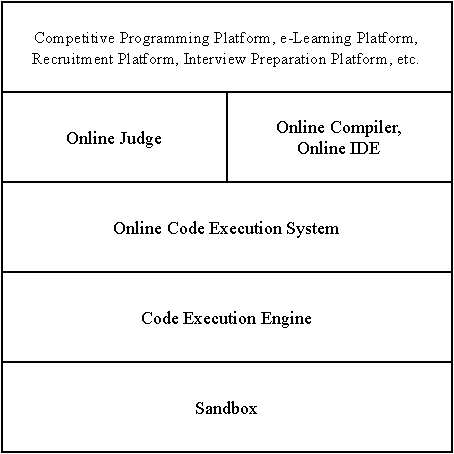
\includegraphics[width=8cm]{images/OJ_ecosystem.pdf}
	\caption{
		Arhitektura OJ ekosistema. \citep{9245310}
	}
	\label{fig:oj-ecosystem}
\end{figure}

Detaljnu klasifikaciju i pregled sustava za udaljeno ocjenjivanje opisuje \citep{wasik2018survey} i njihova zajednička funkcionalnost je procjena \engl{assessment} programskog kôda kojeg korisnik prilaže kao rješenje zadataka, a ocjena \engl{score} programskog kôda koristi se u svrhu koja ovisi o slučaju uporabe.

Najčešća izvedba sustava za udaljeno ocjenjivanje su \textit{web} aplikacije za natjecateljsko programiranje poput: Codeforces \citep{Codeforces}, CodeChef \citep{CodeChef} i SPOJ \citep{SPOJ} gdje se od korisnika očekuje da iz teksta zadatka prepozna i implementira algoritam i odgovarajuću strukturu podataka koji će zadovoljiti zadana vremenska i memorijska ograničenja. 

Izvedba sustava za udaljeno ocjenjivanje kao \textit{web} aplikacije za e-učenje poput \textit{web} aplikacija Edgar \citep{mekterovic2020building} i CodeChum \citep{maranga2019codechum} koristi se za ocjenjivanje \engl{scoring} programskog kôda kojeg student prilaže kao rješenje zadatka iz npr.\ domaće zadaće ili provjere znanja.

\begin{figure}[htb]
	\centering
	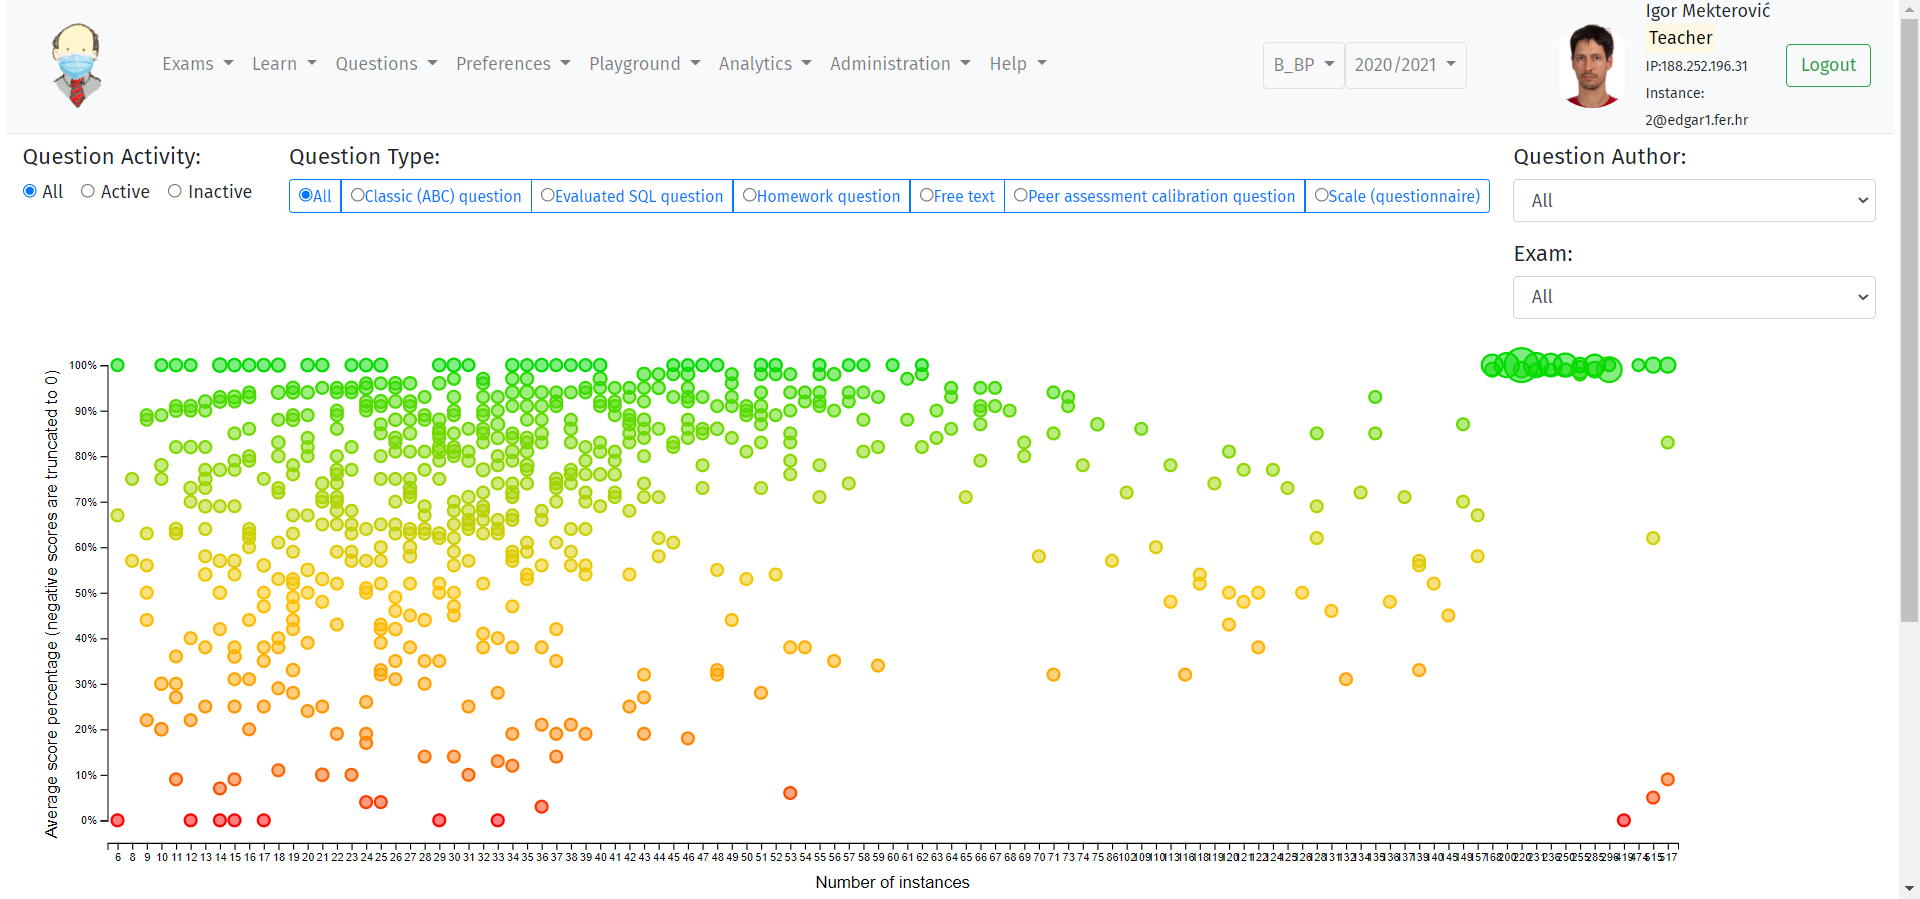
\includegraphics[width=\textwidth]{images/edgar-ui.png}
	\caption{
		Sučelje \textit{web} aplikacije Edgar iz perspektive učitelja.
	}
	\label{fig:edgar-ui}
\end{figure}

\begin{figure}[htb]
	\centering
	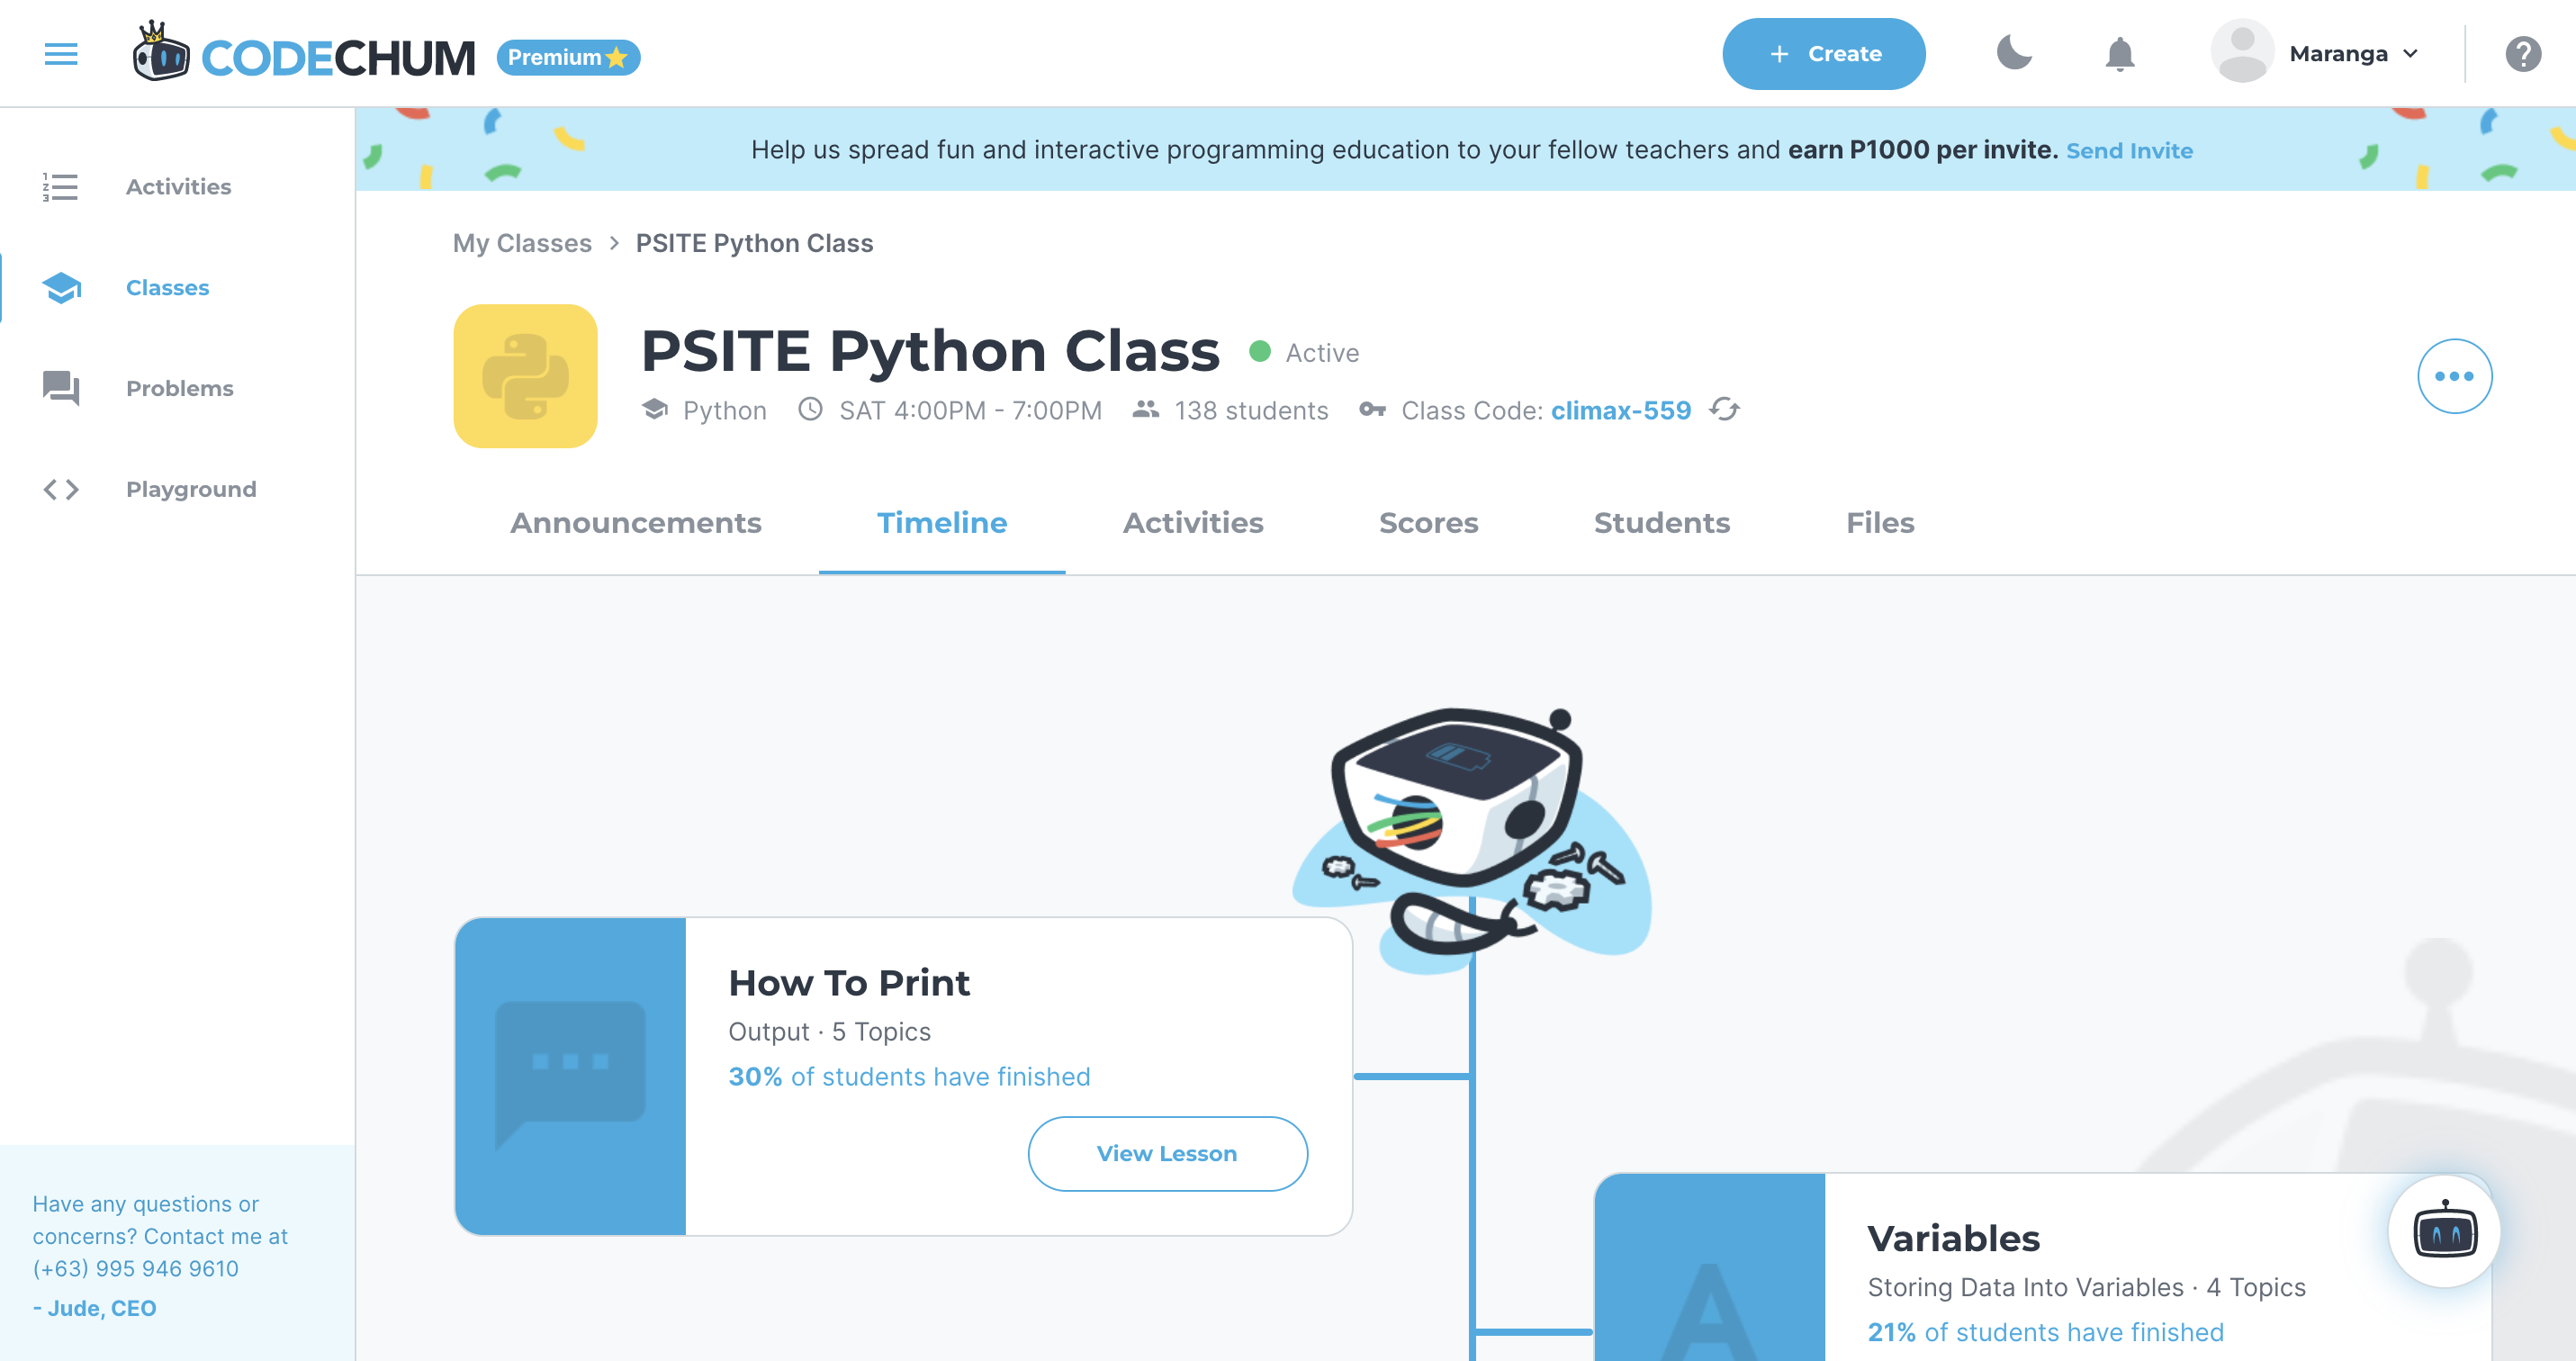
\includegraphics[width=\textwidth]{images/codechum-ui.png}
	\caption{
		Sučelje \textit{web} aplikacije CodeChum.
	}
	\label{fig:codechum-ui}
\end{figure}

\textit{Web} aplikacije poput HackerRank \citep{HackerRank}, TestDome \citep{TestDome} i Filtered \citep{Filtered} koriste se u regrutaciji i procesu zapošljavanja novih softverskih inženjera. Nakon što se prijave na otvorenu poziciju, kandidatima se automatski šalje elektronička pošta s uputama za rješavanje programskih zadataka. Zadatke koje će kandidat rješavati priprema tvrtka za čiju poziciju se kandidat natječe, a težina i vrsta zadataka ovisi o otvorenoj poziciji. Aplikacije za regrutaciju i automatizaciju procesa zapošljavanja najčešće nude svoju biblioteku zadataka koje tvrtke mogu odabrati prilikom izrade ispita za pojedini natječaj. Ovakve \textit{web} aplikacije korisne su tvrtkama koje svakodnevno dobivaju preveliku količinu prijava koje odjel za ljudske resurse može pogledati, stoga im automatizirano ispitivanje kandidata pomaže u inicijalnom filtriranju  prilikom zapošljavanja. Osim filtriranja kandidata ove \textit{web} aplikacije pomažu i pri provođenju \textit{online} razgovora gdje kandidati svoje vještine rješavanja problemskih zadatka trebaju pokazati pred ispitivačem koji vodi razgovor (slika \ref{fig:hackerrank-ui}).

\begin{figure}[htb]
	\centering
	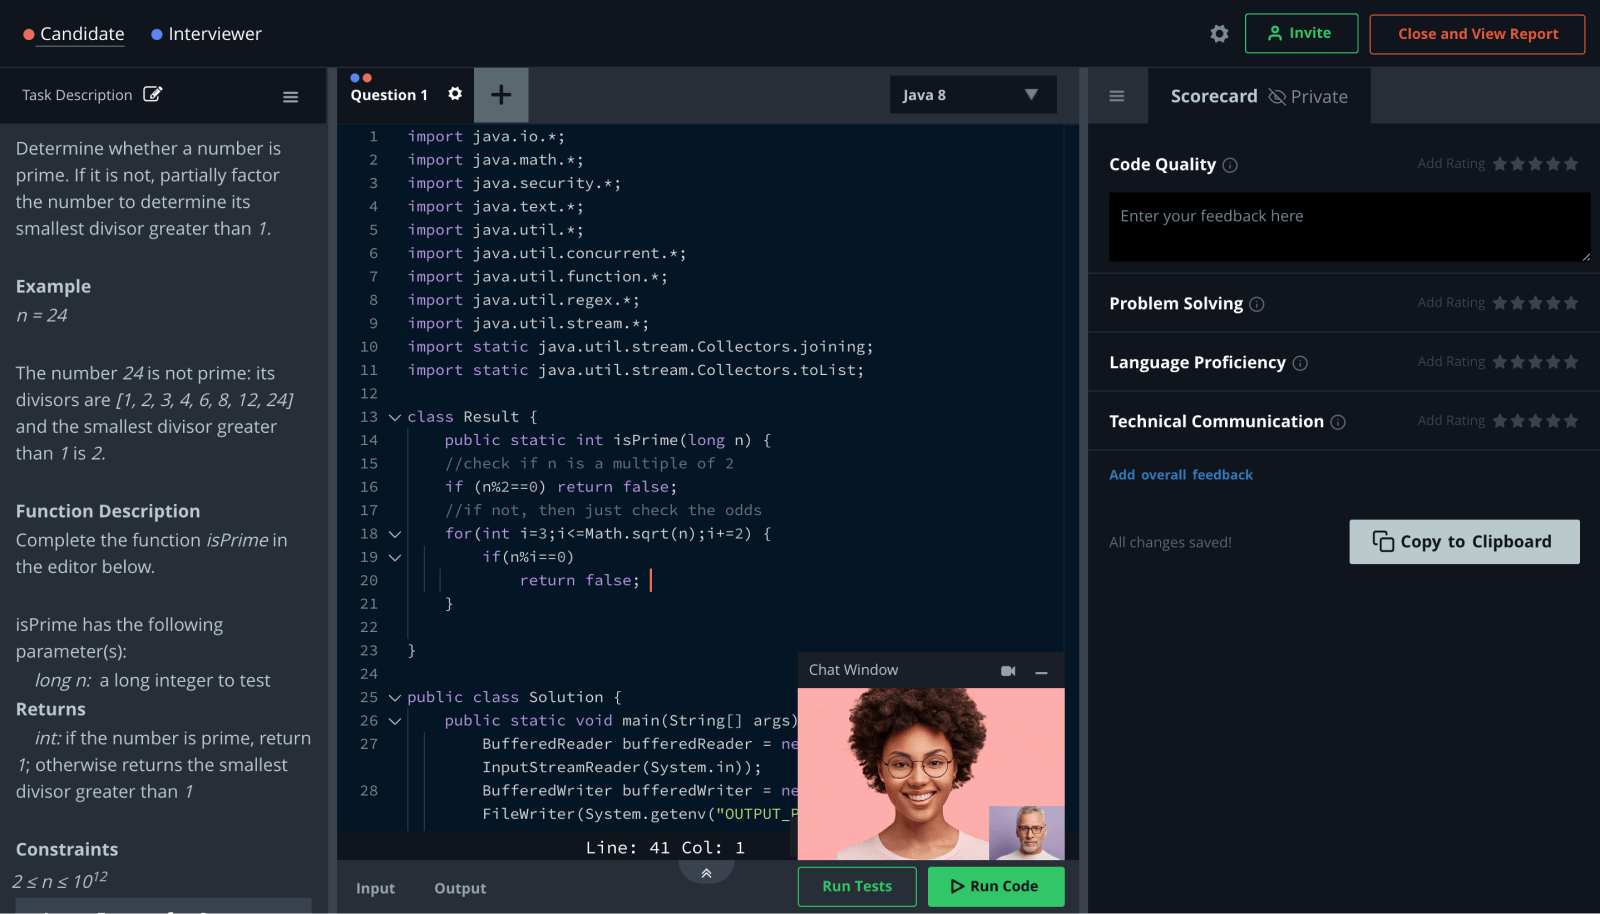
\includegraphics[width=\textwidth]{images/hackerrank-ui.png}
	\caption{
		Sučelje \textit{web} aplikacije HackerRank. \citep{HackerRank}
	}
	\label{fig:hackerrank-ui}
\end{figure}

Osim što pomažu u regrutaciji i procesu zapošljavanja, sustavi za udaljeno ocjenjivanje dolaze i u izvedbi kao \textit{web} aplikacije za vježbanje i pripremu za razgovore za posao koji uključuju rješavanje problemskih zadataka. \textit{Web} aplikacije poput: AlgoExpert \citep{AlgoExpert}, AlgoDaily \citep{AlgoDaily} i LeetCode \citep{LeetCode} svojim korisnicima nude bogatu biblioteku problemskih zadataka, njihovih rješenja i mnogo sadržaja za učenje algoritama i struktura podataka, a sve u svrhu kvalitetne pripreme za tzv. \textit{coding interview}.

\begin{figure}[htb]
	\centering
	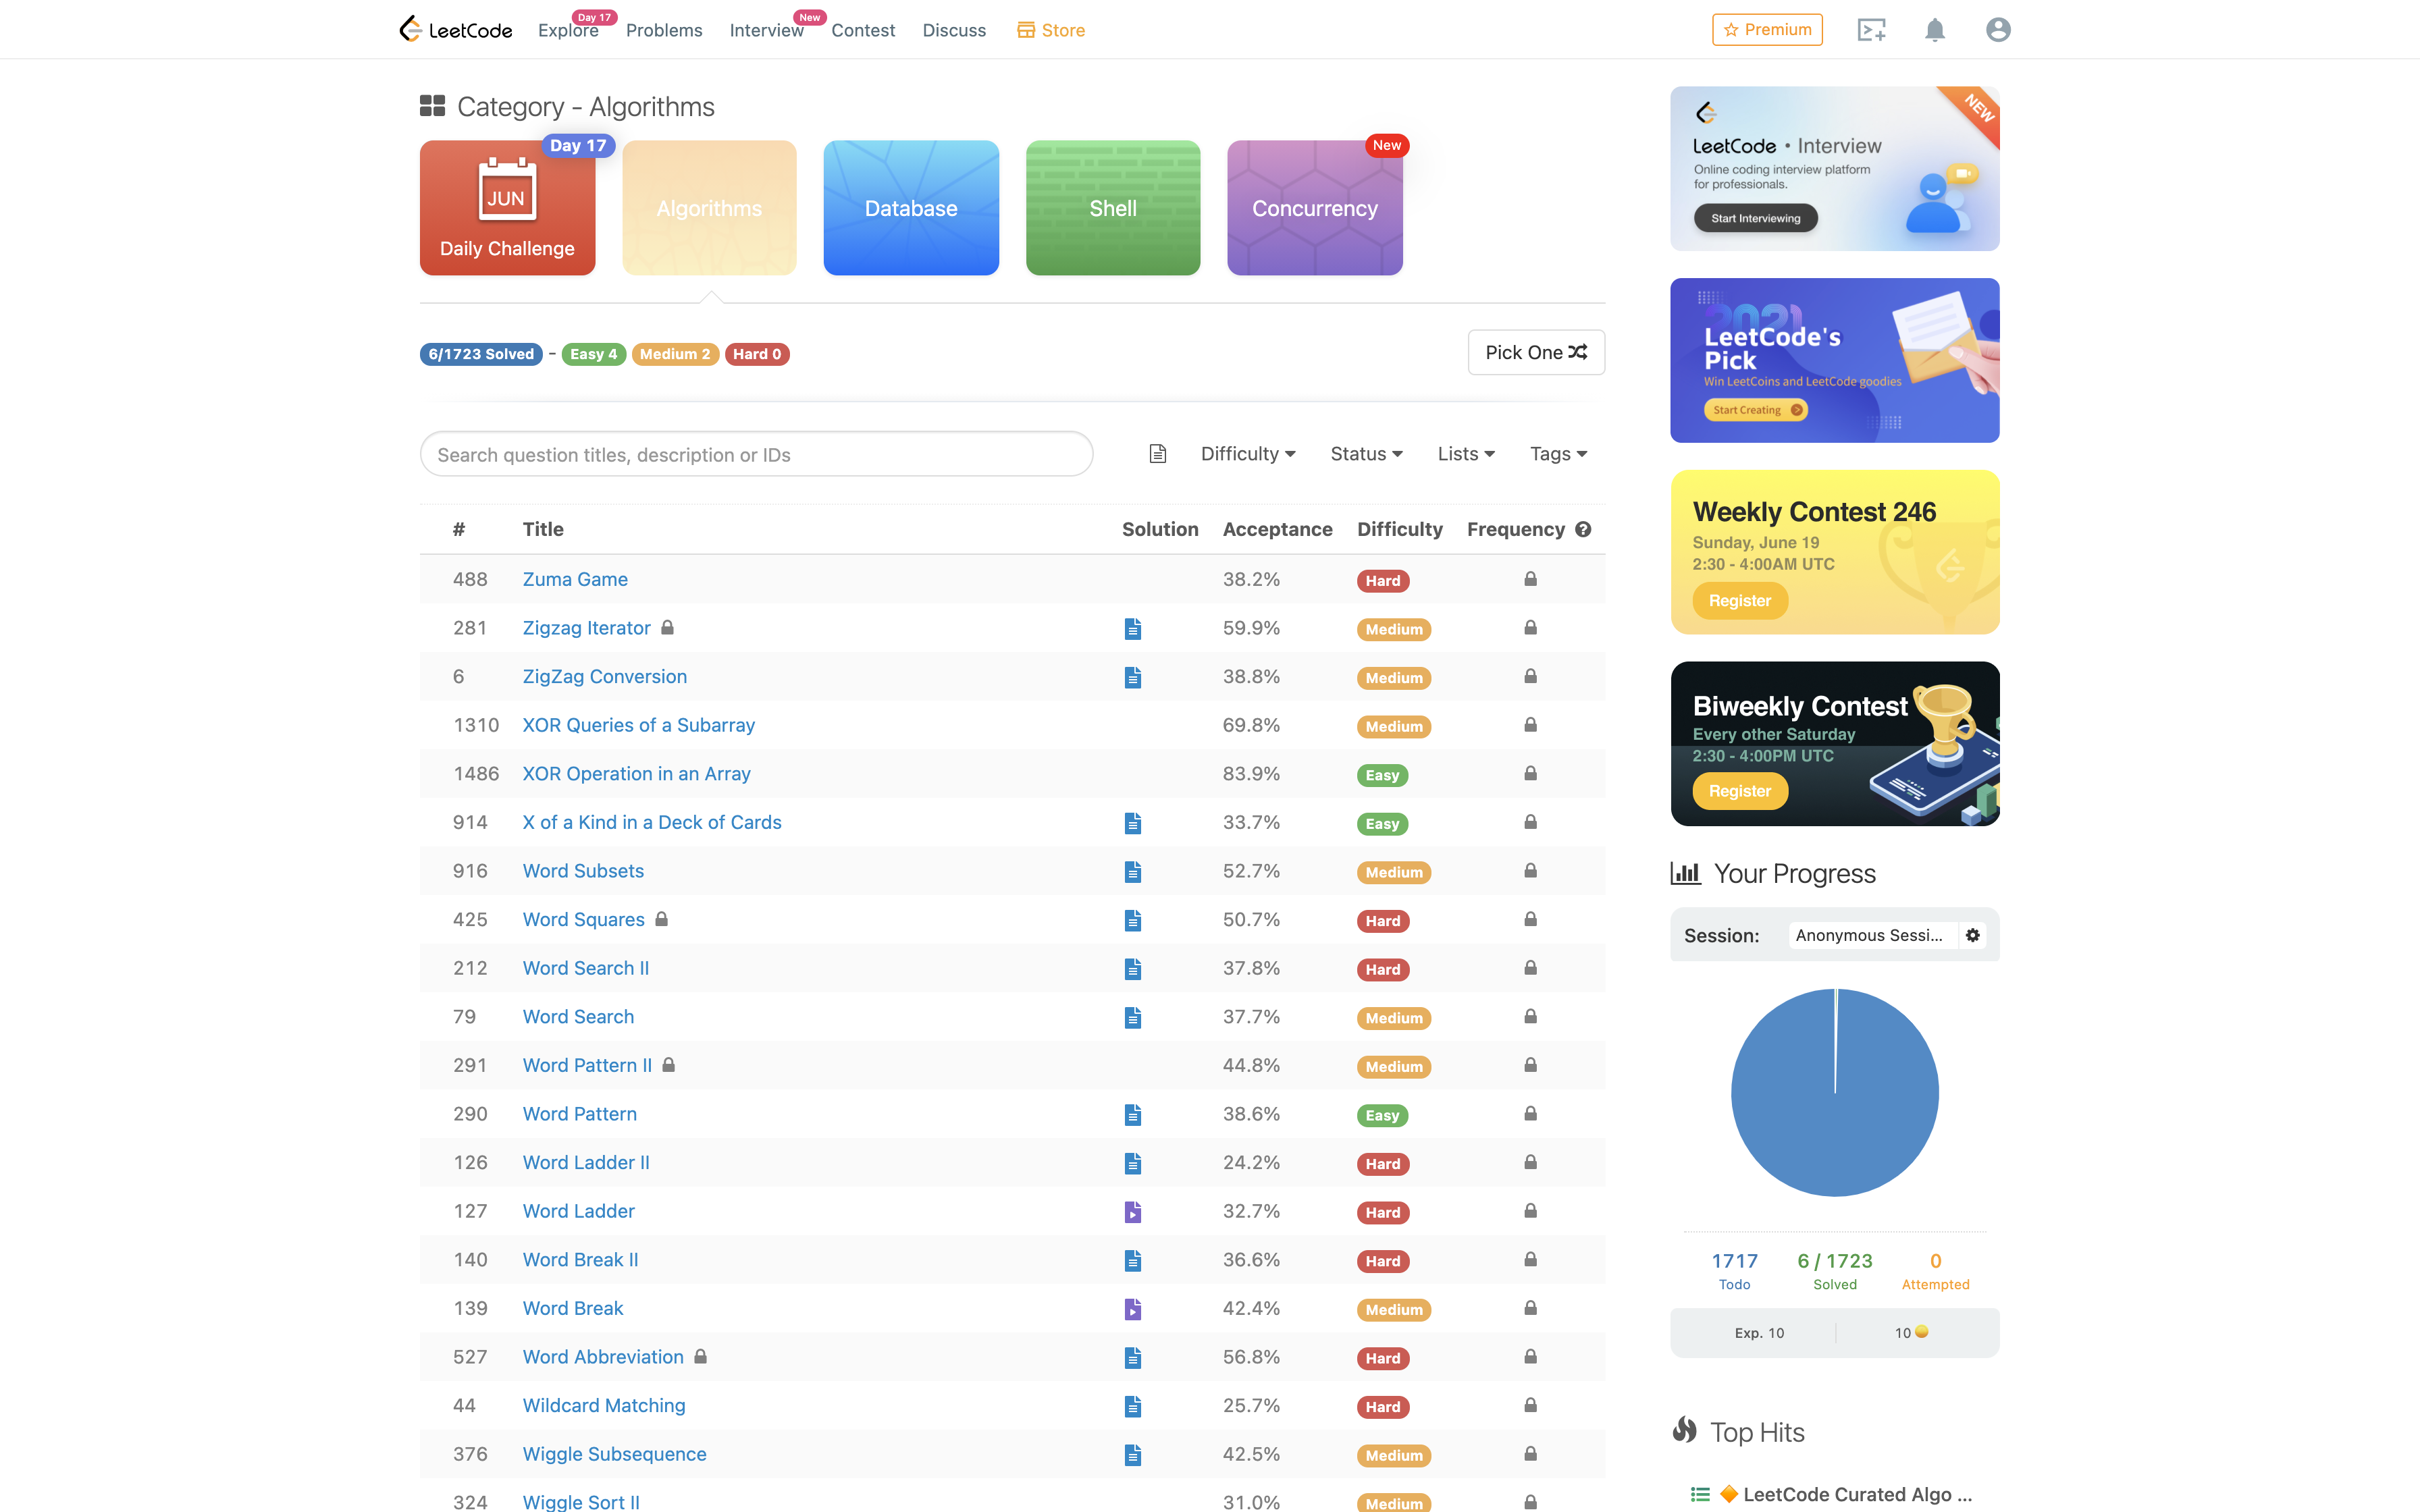
\includegraphics[width=\textwidth]{images/leetcode-ui.png}
	\caption{
		Sučelje \textit{web} aplikacije LeetCode.
	}
	\label{fig:leetcode-ui}
\end{figure}

Pored dosad nabrojanih specijaliziranih aplikacija koje se arhitekturalno oslanjaju na sustav za udaljeno ocjenjivanje (slika \ref{fig:oj-ecosystem}) postoje još i \textit{web} aplikacije za udaljeno programiranje \engl{online compilers} i \textit{web} aplikacije za udaljeno razvijanje \engl{online IDEs}. \textit{Web} aplikacija poput aplikacije Judge0 IDE \citep{Judge0IDE} u izvedbi aplikacije za udaljeno programiranje omogućuje korisniku pisanje, prevođenje i izvršavanje programskog kôda u jednom od podržanih programskih jezika (slika \ref{fig:judge0-ide-ui}). \citep{wasik2018survey} daje detaljnu usporedba ovakvih i sličnih \textit{web} aplikacija.

\begin{figure}[htb]
	\centering
	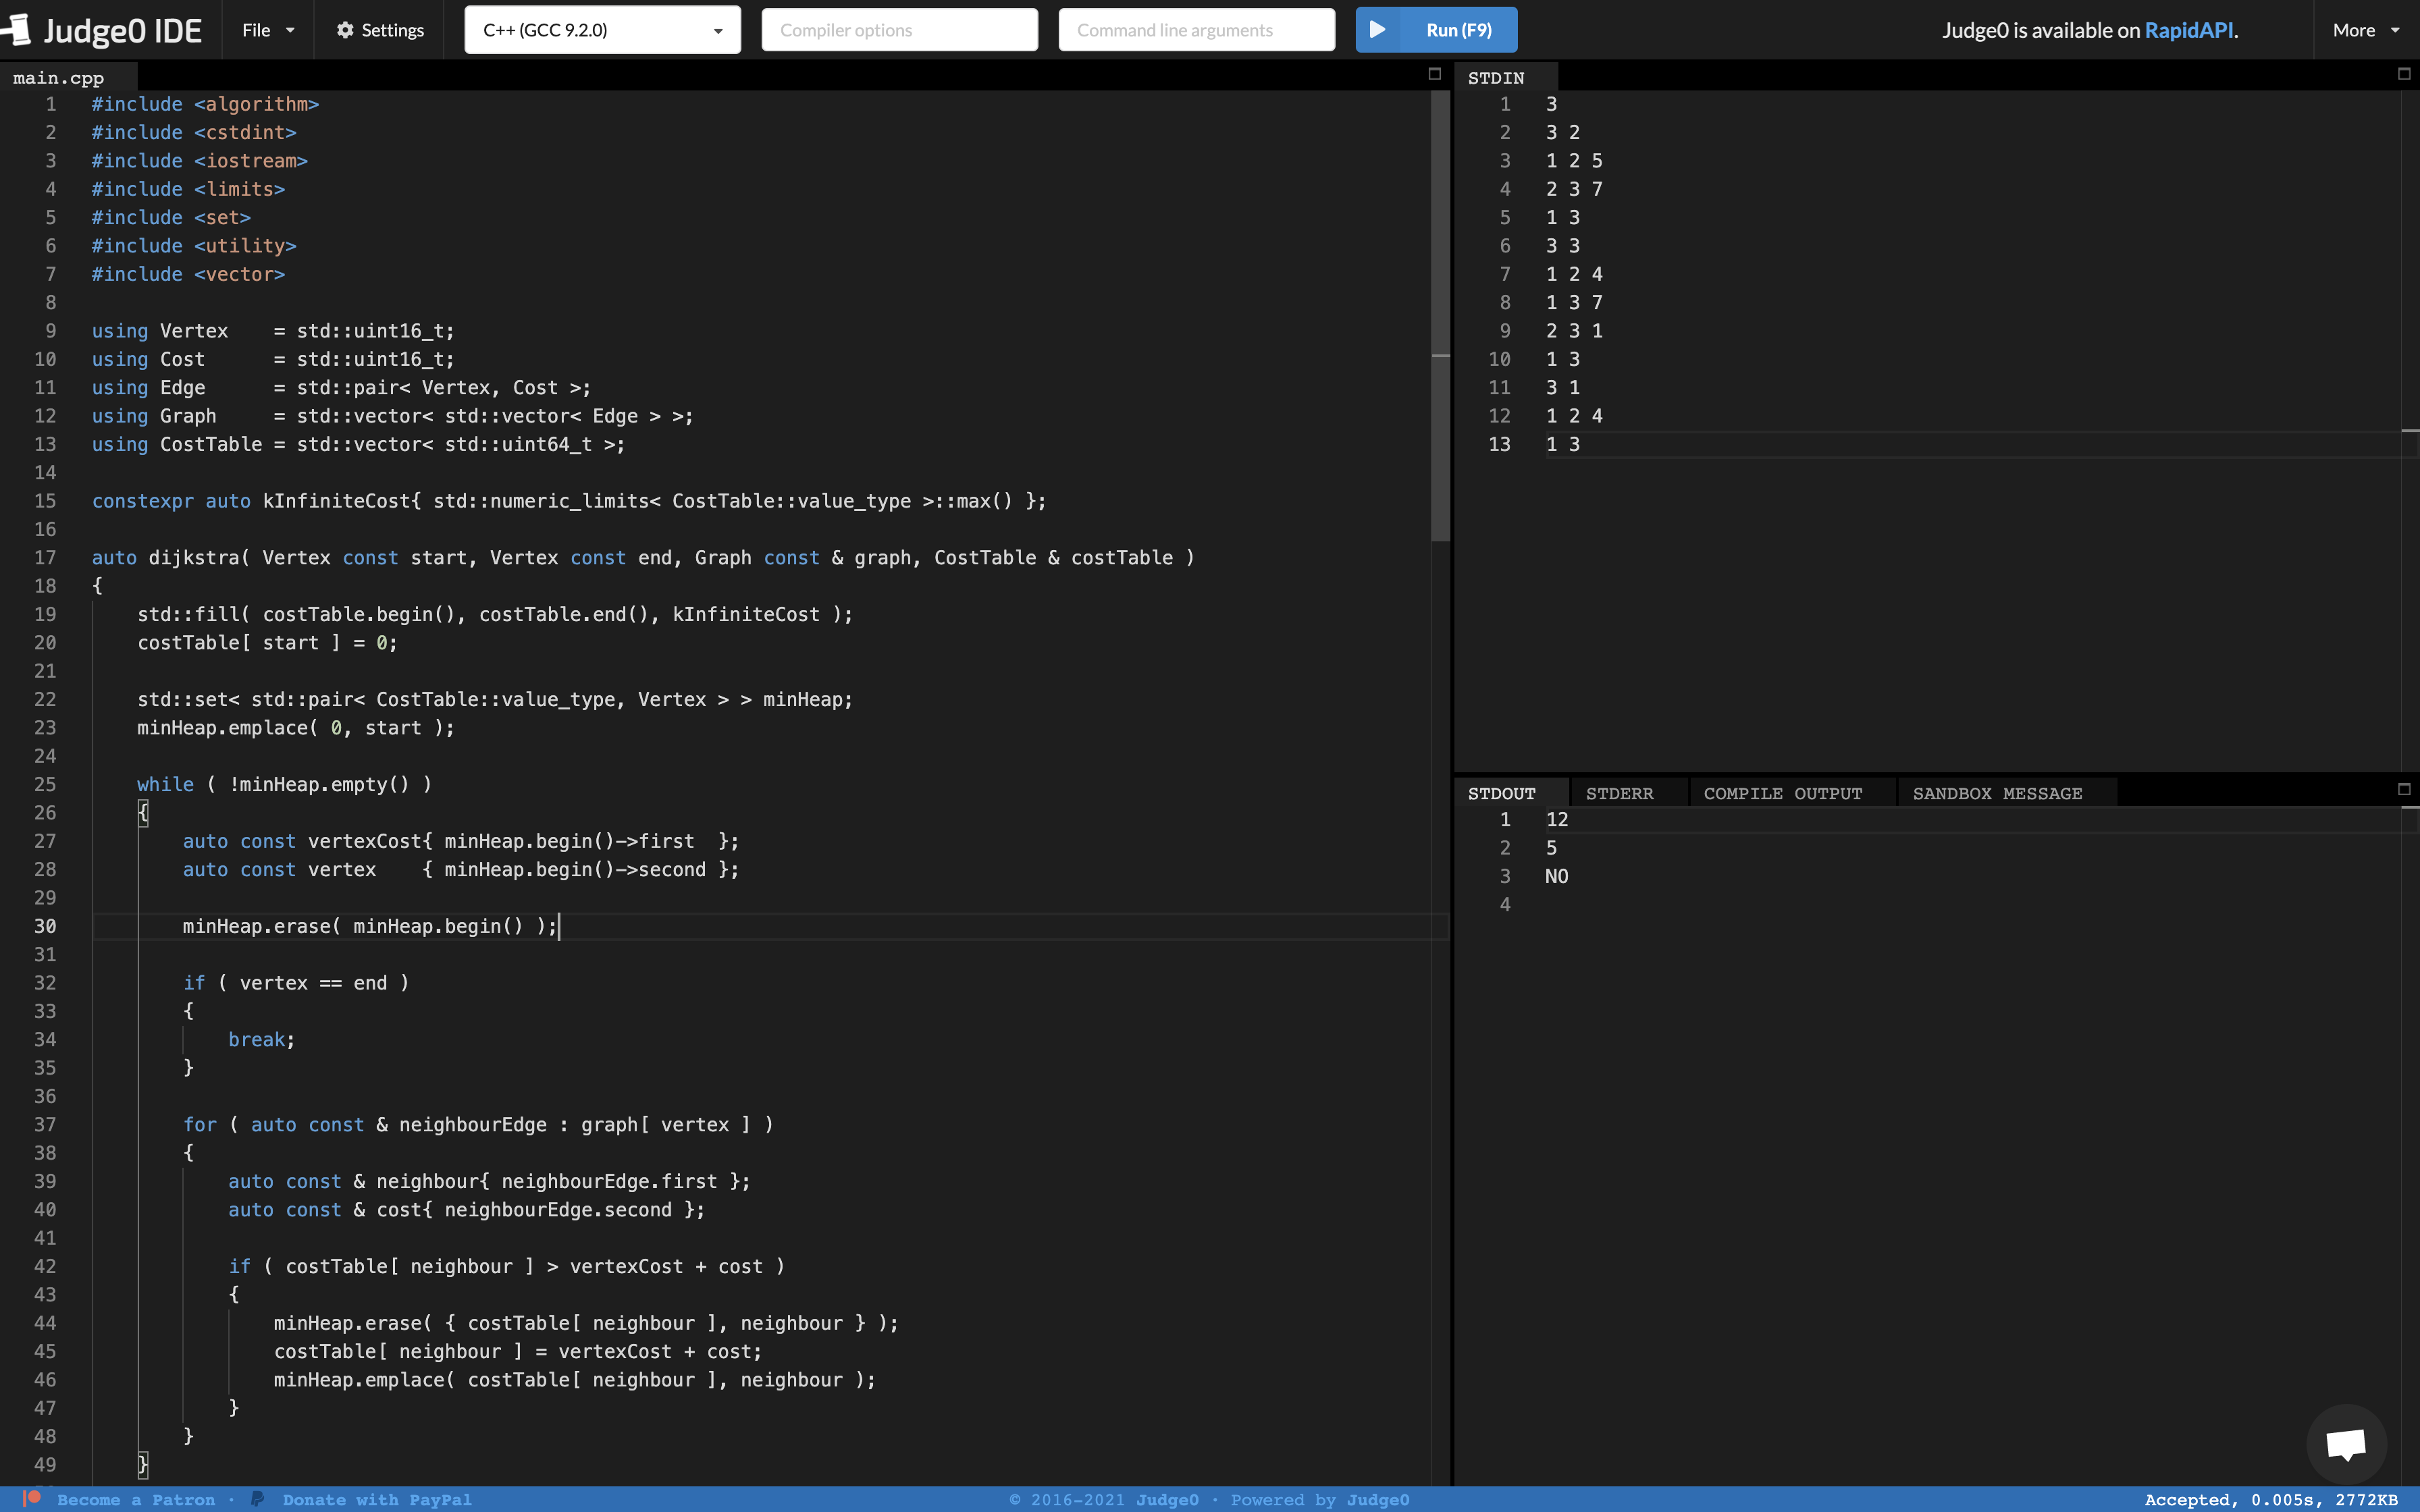
\includegraphics[width=\textwidth]{images/judge0-ide-ui.png}
	\caption{
		Sučelje \textit{web} aplikacije Judge0 IDE.
	}
	\label{fig:judge0-ide-ui}
\end{figure}

Formalno, sustav za udaljeno ocjenjivanje \citep{wasik2018survey} definira kao udaljenu uslugu \engl{online service} koja u oblaku \engl{cloud} izvodi barem jednu od sljedećih faza:
\begin{itemize}
    \item podnošenje zahtjeva za izvršavanje programskog kôda \engl{submission},
    \item procjena podnesenoga programskog kôda \engl{assessment},
    \item ocjenjivanje podnesenoga programskog kôda \engl{scoring}.
\end{itemize}

Podnošenje zahtjeva za izvršavanje programskog kôda podrazumijeva prihvaćanje programskog kôda u sustav, prevođenje po potrebi i verifikaciju da je program spreman za izvršavanje. U procjeni podnesenoga programskog kôda program se pokreće za svaki ispitni primjer i provjerava se uspješnost izvođenja programa u zadanim vremenskim i memorijskim ograničenjima. Također, u istoj fazi, provjerava se standardni izlaz \engl{standard output} korisničkog programa i uspoređuje ga se s očekivanim izlazom za trenutni ispitni primjer \engl{expected output}. Konačno, u fazi ocjenjivanja, podnesenom programskom kôdu dodjeljuje se ocjena na temelju rezultata iz prethodnih faza. Tako npr.\ na ocjenu u natjecateljskom programiranju može utjecati vrijeme koje je bilo potrebno natjecatelju da riješi pojedini zadatak. Što kasnije natjecatelj riješi ispravno zadatak to će manje bodova dobiti čak i ako su mu svi ispitni primjeri ispravni uz zadana vremenska i memorijska ograničenja.

\section{Udaljeno izvođenje programskog kôda}
Prethodno poglavlje, koje daje pregled svega nekoliko najčešćih slučajeva uporabe sustava za udaljeno ocjenjivanje, također daje naslutiti da se za svaki slučaj uporabe programski kôd korisnika mora negdje prevesti i izvesti. Najjednostavnije rješenje ovog problema bilo bi da korisnik samostalno prevede i izvede svoj program, i da zatim u sustav postavi rješenja koja je dobio. Ovakav pristup bio bi u redu za napredne korisnike koji znaju instalirati i koristiti odgovarajući prevoditelj za odabrani programski jezik, međutim, za početnike ovakav bi pristup bio jako loše korisničko iskustvo. Međutim, ovo nije jedini argument zašto nije dobro da korisnik samostalno prevodi, izvodi i postavlja rješenja svog programa. Ispitni primjeri trebaju ostati nepoznati korisniku kako ih korisnik ne bi zloupotrijebio. Korisnik ne treba znati očekivani izlaz svog programa da bi ga zloupotrijebio, za neke zadatke dovoljno je imati standardni ulaz \engl{standard input} iz kojeg se lako dobije očekivani izlaz. Već se samo sa ovim snažno opravdanim zahtjevom može zaključiti da je programski kôd korisnika potrebno izvršiti na poslužitelju kojem korisnik nema pristup. Ovakav zahtjev otvara novi spektar problema koje je potrebno riješiti i koji su opisani u \citep{kurnia2001online}.

Pokretanje programskog kôda korisnika na udaljenom poslužitelju nameće izazov da se korisnikov program mora pokrenuti u zaštićenom okruženju \engl{sandboxed environment} kako ne bi negativno utjecao na rad poslužitelja i ostalih procesa. Postoje razne tehnike opisane u \citep{yi2014comparison} koje se za to koriste, a u kontekstu sustava za udaljeno ocjenjivanje od zaštićenog okruženja očekujemo sljedeće funkcionalnosti:
\begin{itemize}
    \item inicijalizaciju zaštićenog okruženja,
    \item mogućnost prenošenja programskog kôda korisnika u zaštićeno okruženje,
    \item prevođenje i izvođenje programskog kôda u zaštićenom okruženju uz navedena vremenska i memorijska ograničenja,
    \item prikupljanje izlaza programa i meta podatka o izvođenju, i
    \item uništavanje zaštićenog okruženja.
\end{itemize}

Važnost korištenja zaštićenog okruženja koje osigurava da programski kôd korisnika ne šteti radu poslužitelja i ostalih procesa prikazuju isječci \ref{lst:infinite-compilation} i \ref{lst:fork-bomb} napisani u programskom jeziku C. 

Isječak \ref{lst:infinite-compilation} prikazuje ispravan C program koji uključuje uređaj pseudo-slučajnih brojeva sustava Linux. Budući da uređaj generira beskonačni slijed pseudo-slučajnih brojeva, uključivanje tog uređaja u programu dovodi do beskonačnog vremena prevođenja. Ukoliko više korisnika napravi zahtjev za izvođenjem ovakvog ili sličnog programa na poslužitelju, brzo dolazi do iscrpljivanja računskih i memorijskih resursa na poslužitelju i time poslužitelj postaje neupotrebljiv.
Iz ovog je jednostavnog primjera jasno da je potrebno proces prevođenja izolirati u zaštićeno okruženje koje će imati ograničene vremenske i memorijske resurse.

\begin{lstlisting}[
    caption={Ispravan C program s beskonačnim vremenom prevođenja.},
    label={lst:infinite-compilation},
    language=c
]
#include </dev/random>
int main() {
    return 0;
}
\end{lstlisting}

Izoliranje izvršavanja programskog kôda korisnika još je važnije od izolacije prevođenja, budući da je za zloupotrebu neizoliranog procesa prevođenja potrebno nešto više znanja o prevodiocima i programskom jeziku koji se koristi. Isječak \ref{lst:fork-bomb} prikazuje C program koji će beskonačno mnogo puta stvoriti novi proces, i svaki novostvoreni proces napravit će isto. Budući da se broj novostvorenih procesa može opisati eksponencijalnom funkcijom $f(x) = 2^x$, gdje je $x$ broj ponavljanja petlje, ovaj program naziva se \textit{fork bomb}. Dovoljno je da jedan korisnik pokrene ovakav program da se na poslužitelju iscrpe računski i memorijski resursi koji će ga učiniti neupotrebljivim.

\begin{lstlisting}[
    caption={C program s beskonačnim grananjem novih procesa.},
    label={lst:fork-bomb},
    language=c
]
#include <unistd.h>
int main() {
    while(1) {
        fork();
    }
    return 0;
}
\end{lstlisting}

Oba isječka još jednom potvrđuju da je u sustavima za udaljeno ocjenjivanje nužno koristiti zaštićenu okolinu koja će prevoditi i izvršavati programski kôd svakog korisnika. Gledajući iz perspektive sustava za udaljeno ocjenjivanje svaki programski kôd korisnika smatra se opasnim, stoga se u kontekstu sustava za udaljeno ocjenjivanje govori o nepovjerljivom programskom kôdu \engl{untrusted source code} kojeg je potrebno prevesti i izvršiti.

\section{Sustavi za udaljeno izvršavanje programskog kôda}
Sustav za udaljeno izvršavanje programskog kôda (engl.\ \textit{online code execution system}, krat.\ \textit{OCES}) je sustav koji nudi \textit{web} aplikacijsko sučelje \engl{web API} za prevođenje i izvršavanje proizvoljnog programskog kôda. Arhitekturalni prikaz na slici \ref{fig:oj-ecosystem} izdvaja sustav za udaljeno izvršavanje programskog kôda kao zasebnu komponentu na koju se oslanjaju sustav za udaljeno ocjenjivanje, a zatim i sustavi razvijeni za specifičan slučaj uporabe.

Formalno, \citep{9245310} definira sustav za udaljeno izvršavanje programskog kôda kroz funkcionalne i ne funkcionalne zahtjeve.

\subsection{Arhitektura sustava za udaljeno izvršavanje programskog kôda}
\subsection{Sustav Judge0}
\subsection{Sustav Piston}
\subsection{Sustav Sphere Engine}

\chapter{Analiza sustava za udaljeno izvršavanje programskog kôda}

\chapter{Sustav Hélory}
\section{Specifikacija zahtjeva}
\section{Korištene tehnologije}
\section{Programska izvedba}
\section{Pregled sučelja}

\chapter{Primjer korištenja sustava Hélory u analizi sustava Judge0}

\chapter{Budući razvoj sustava Hélory}

\chapter{Zaključak}

\bibliography{literatura}
\bibliographystyle{fer}

\begin{sazetak}
\kljucnerijeci{Ključne riječi, odvojene zarezima.}
\end{sazetak}

\engtitle{Performance analysis of online code execution systems}
\begin{abstract}
\keywords{Keywords.}
\end{abstract}

\end{document}
